
\chapter*{Coloring}
\label{chap:coloring}

As a reward that you have have read this far you can color some \lsystems!
You can try to color the \lsystems with the fewest number of colors so that no two adjacent cells will have same color.

\vspace{2cm}

\begin{figure}[h]
	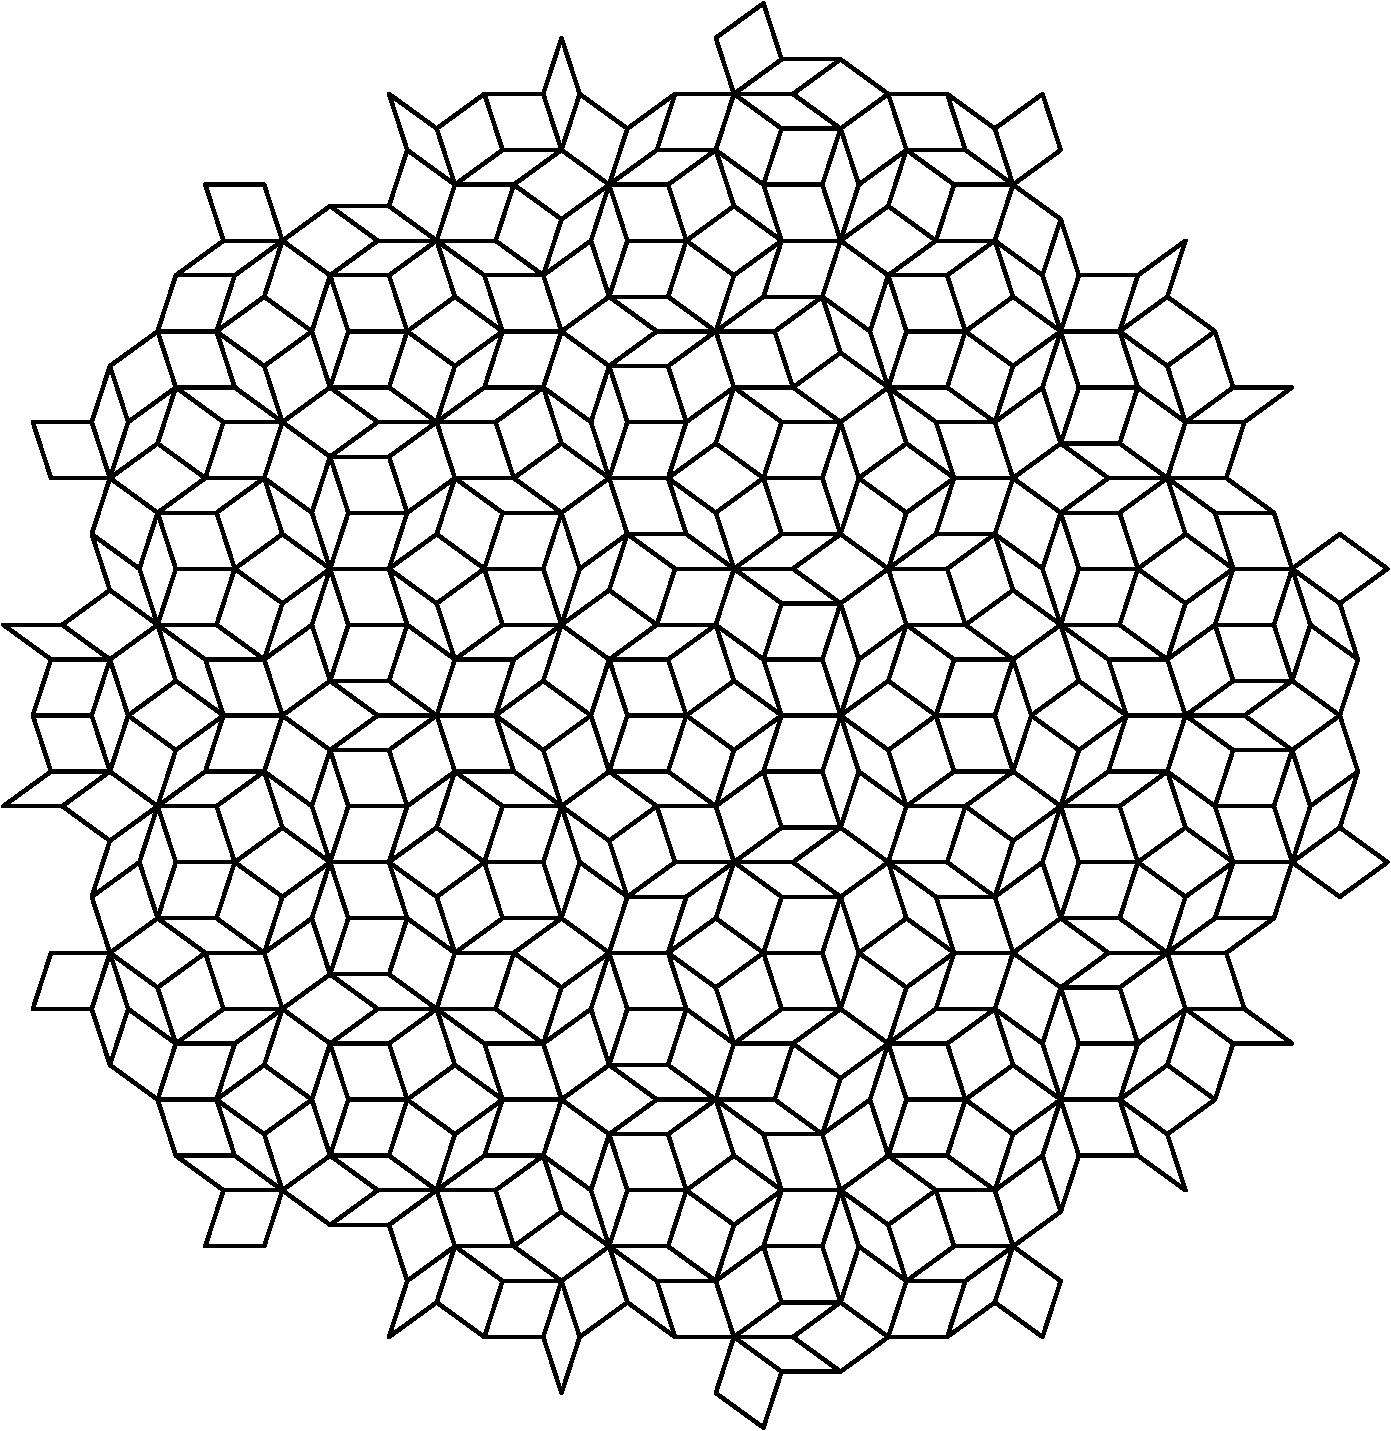
\includegraphics[width=\linewidth]{PenroseColoring}
\end{figure}

\vfill

\begin{figure}[p]
	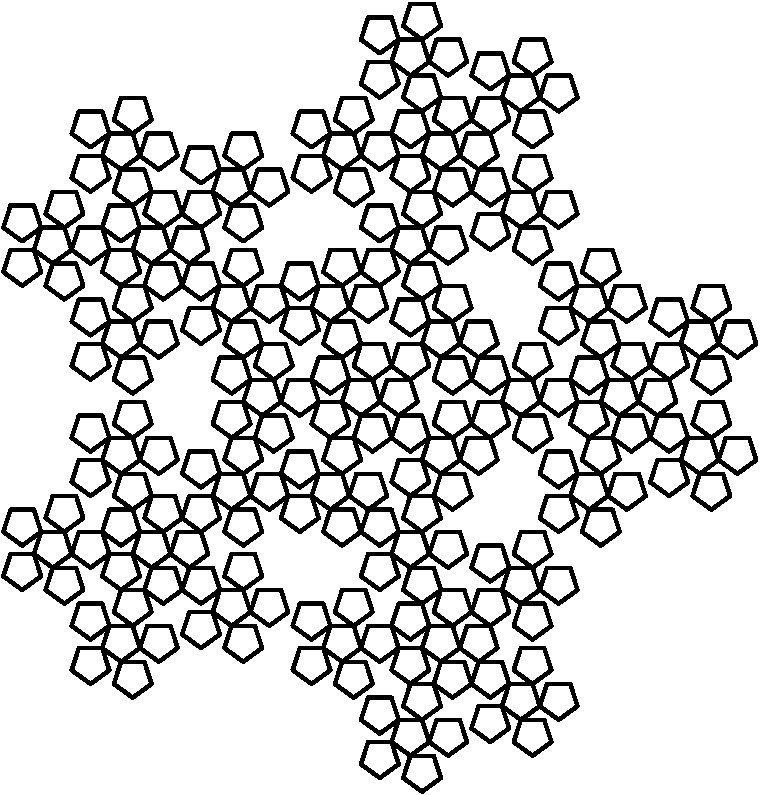
\includegraphics[width=\linewidth]{PentigreeColoring}
\end{figure}

\vfill

\begin{figure}[p]
	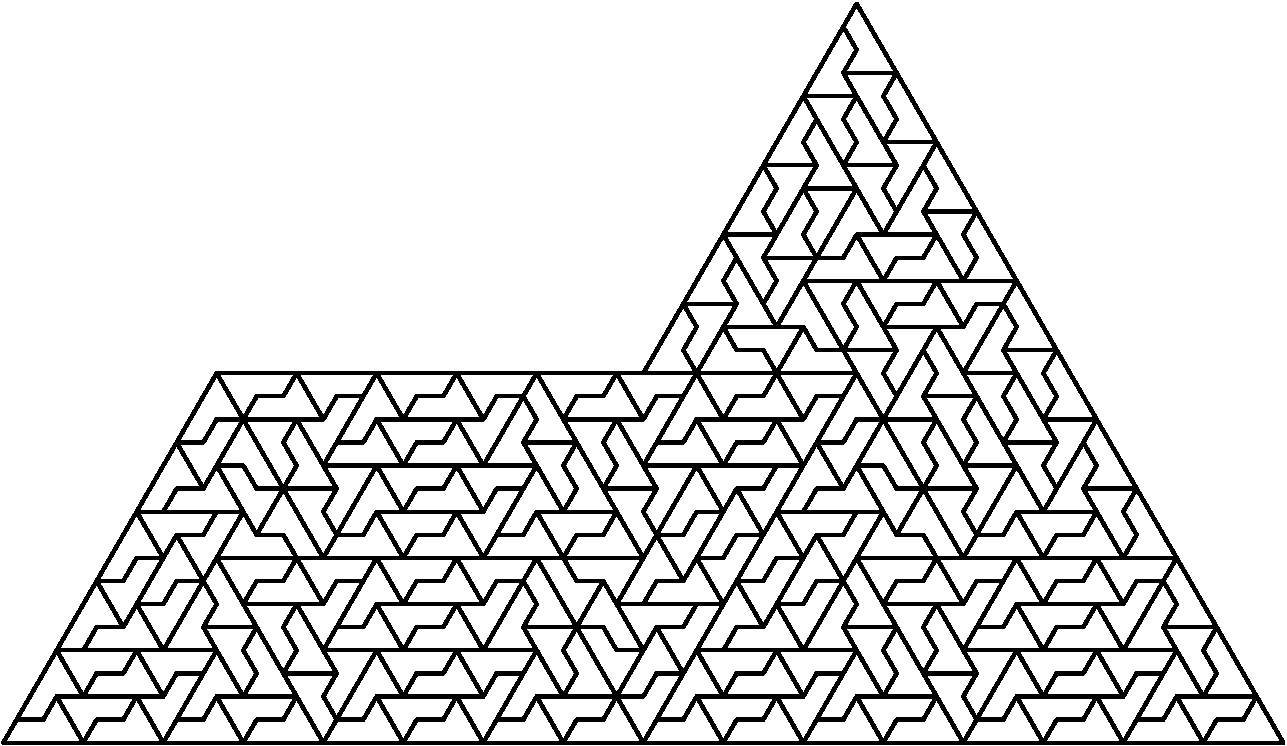
\includegraphics[width=\linewidth]{SphinxForColoring}
\end{figure}

\vfill

\begin{figure}[p]
	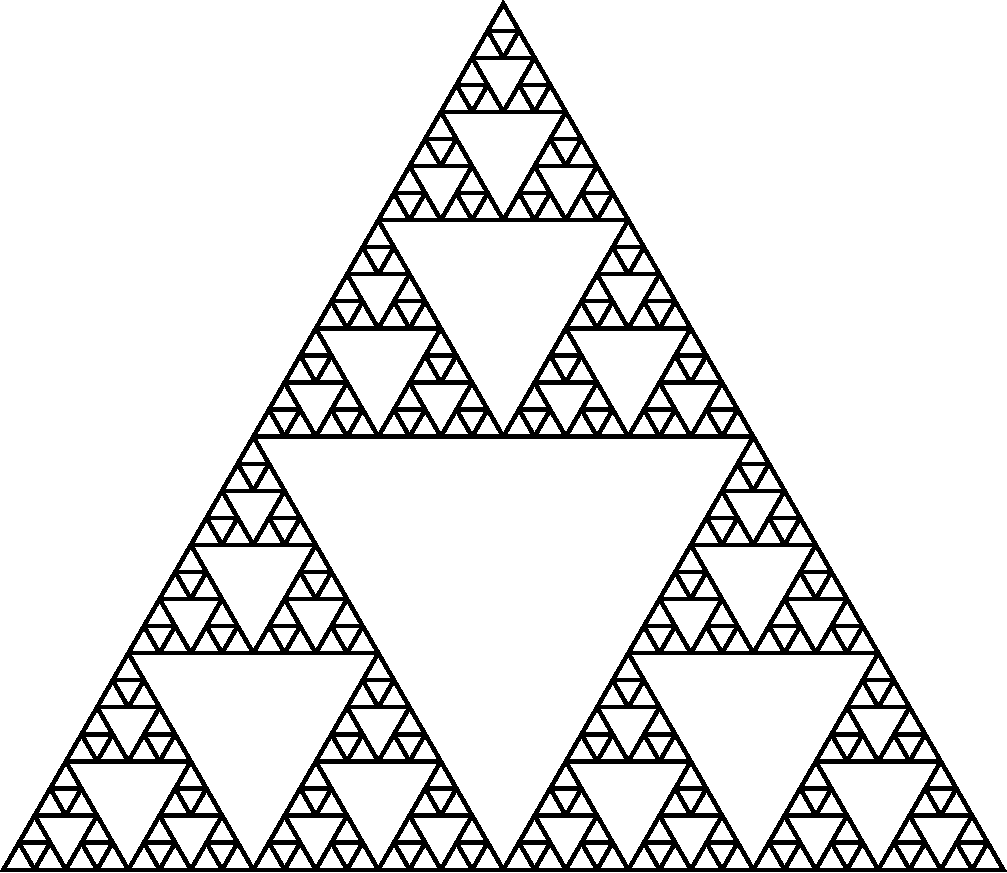
\includegraphics[width=\linewidth]{SierpinskiTriangleColoring}
\end{figure}

\vfill

\begin{figure}[p]
	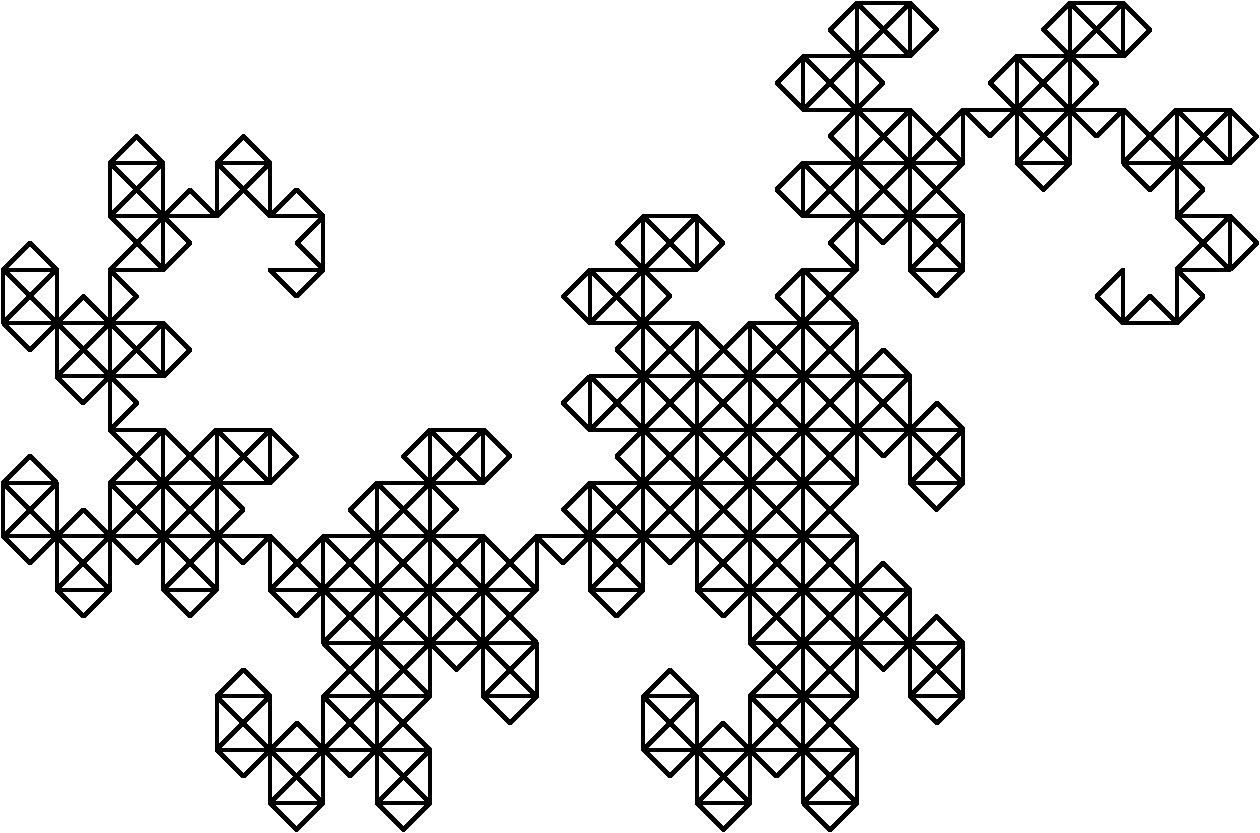
\includegraphics[width=\linewidth]{DragonCurveColoring}
\end{figure}

\vfill







